\begin{center}
  \textbf{Отчёт лабораторной работы №\envReportLabNumber}
\end{center}

\textbf{Тема}:
<<\envReportTitle>>

\textbf{Цель}: ...

% = = = = = = = = = = = = = = = =

\begin{center}
  \textbf{Задание 1}
\end{center}

\textbf{Условие}:
Компания «ПЕГМЕНТ» производит краску для внутренних и наружных работ из сырья двух типов А и В,
которая поступает в оптовую продажу.
Нормативный расход сырья для производства краски и получаемый доход от ее продажи представлен на рисунке~\ref{fig:task1_1}.

\begin{figure}[!htb]
  \centering

  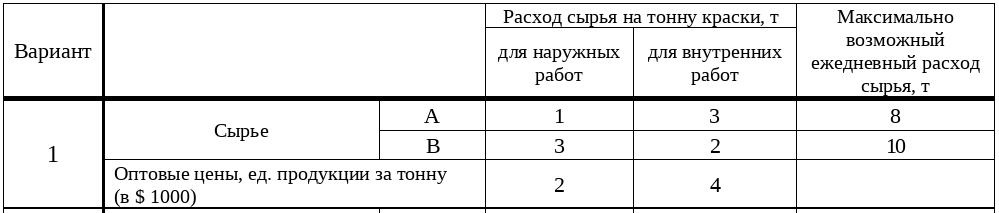
\includegraphics[width=16cm]
  {inc/task1_1.png}

  \caption{Задание 1 вариант 1}
  \label{fig:task1_1}
\end{figure}

Из-за отсутствия надлежащего спроса отдел маркетинга компании ограничил ежедневное производство краски для внутренних работ
до 2 т. и поставил условие,
чтобы ежедневное производство краски для наружных работ не превышало более чем на тонну
аналогичный показатель краски для внутренних работ.
Максимально-возможный ежедневный расход сырья определяется его возрастающим спросом и возможностями складского хранения.

Встает проблема в производстве количества каждого вида продукции с учетом максимизации дохода, реализуемой продукции?

\textbf{Решение}:

$x_1$ - ежедневный объем производства краски для наружных работ;

$x_2$ - ежедневный объем производства краски для внутренних работ.

$$
\begin{cases}
  y = 2 x_1 + 4 x_2 \implies max &\text{- ежедневный доход от продажи}\\
  1 x_1 + 3 x_2  \leq 8 &\text{- ограничение для ежедневного расходы сырья A}\\
  3 x_1 + 2 x_2 \leq 10 &\text{- ограничение для ежедневного расходы сырья B}\\
  x_2 \leq 0 &\text{- ограничение ежедневного производства краски}\\
  &\text{  для внутренних работ}\\
  x_1 \leq x_2 + 1 &\text{- ограничение, чтобы ежедневное производство краски}\\
  &\text{  для наружных работ не превышало более чем на одну тонну}\\
  &\text{  аналогичный показатель краски для внутренних работ}\\
  x_1 \geq 0&\text{- условие не отрицательности переменной}\\
  x_1 \geq 0&\text{- условие не отрицательности переменной}
\end{cases}
$$

\newpage

\begin{center}
\textbf{Решение системы через WinQSB}
\end{center}

На VirtualBox \cite{VirtualBox} устанавливаем WinXP \cite{WinXP}, а на неё программу WinSQB \cite{WinQSB}.

Пуск > WinQSB > Linear and Integer Programming > File > New Problem

Problem Title: MO.PO4.190333-01\_01

Number of Variables: 2

Number of Constraints: 6

Object Criterion > Maxamization

OK> Заполняем таблицу (см.таблицу~\ref{tab:1_1})

\begin{table}[h!]
  \scriptsize

  \centering

  \caption{Решение задачи №1 (вариант 1) в WinQSB (Linear and Integer Programming)}
  \label{tab:1_1}

  \begin{tabular}{ |l||c|c|c|c| } 
    \hline
    Variable & X1 & X2 & Direction & R. H. S \\ \hline
    \hline
    Maximaze & 2 & 4 &  & \\ \hline
    C1 & 1 & 3 & <= & 8 \\ \hline
    C2 & 3 & 2 & <= & 10 \\ \hline
    C3 & 0 & 1 & <= & 2 \\ \hline
    C4 & 1 & -1 & <= & 1 \\ \hline
    C5 & 1 & 0 & >= & 0 \\ \hline
    C6 & 0 & 1 & >= & 0 \\ \hline
    %LowerBound & 0 & 0 &  & \\ \hline
    %UpperBound & M & M &  & \\ \hline
    %VariableType & Continious & Continious &  & \\ \hline
  \end{tabular}
\end{table}

Жмем розовую кнопку > ОК

Options > Change XY Ranges and Colors > Background (жмем, пока не получим белый цвет) > ОК

Options > Change XY Variables > OK

File > Save As > 1.bmp. Результат на рисунке~\ref{fig:result1_option1}.

\begin{figure}[!htb]
  \centering

  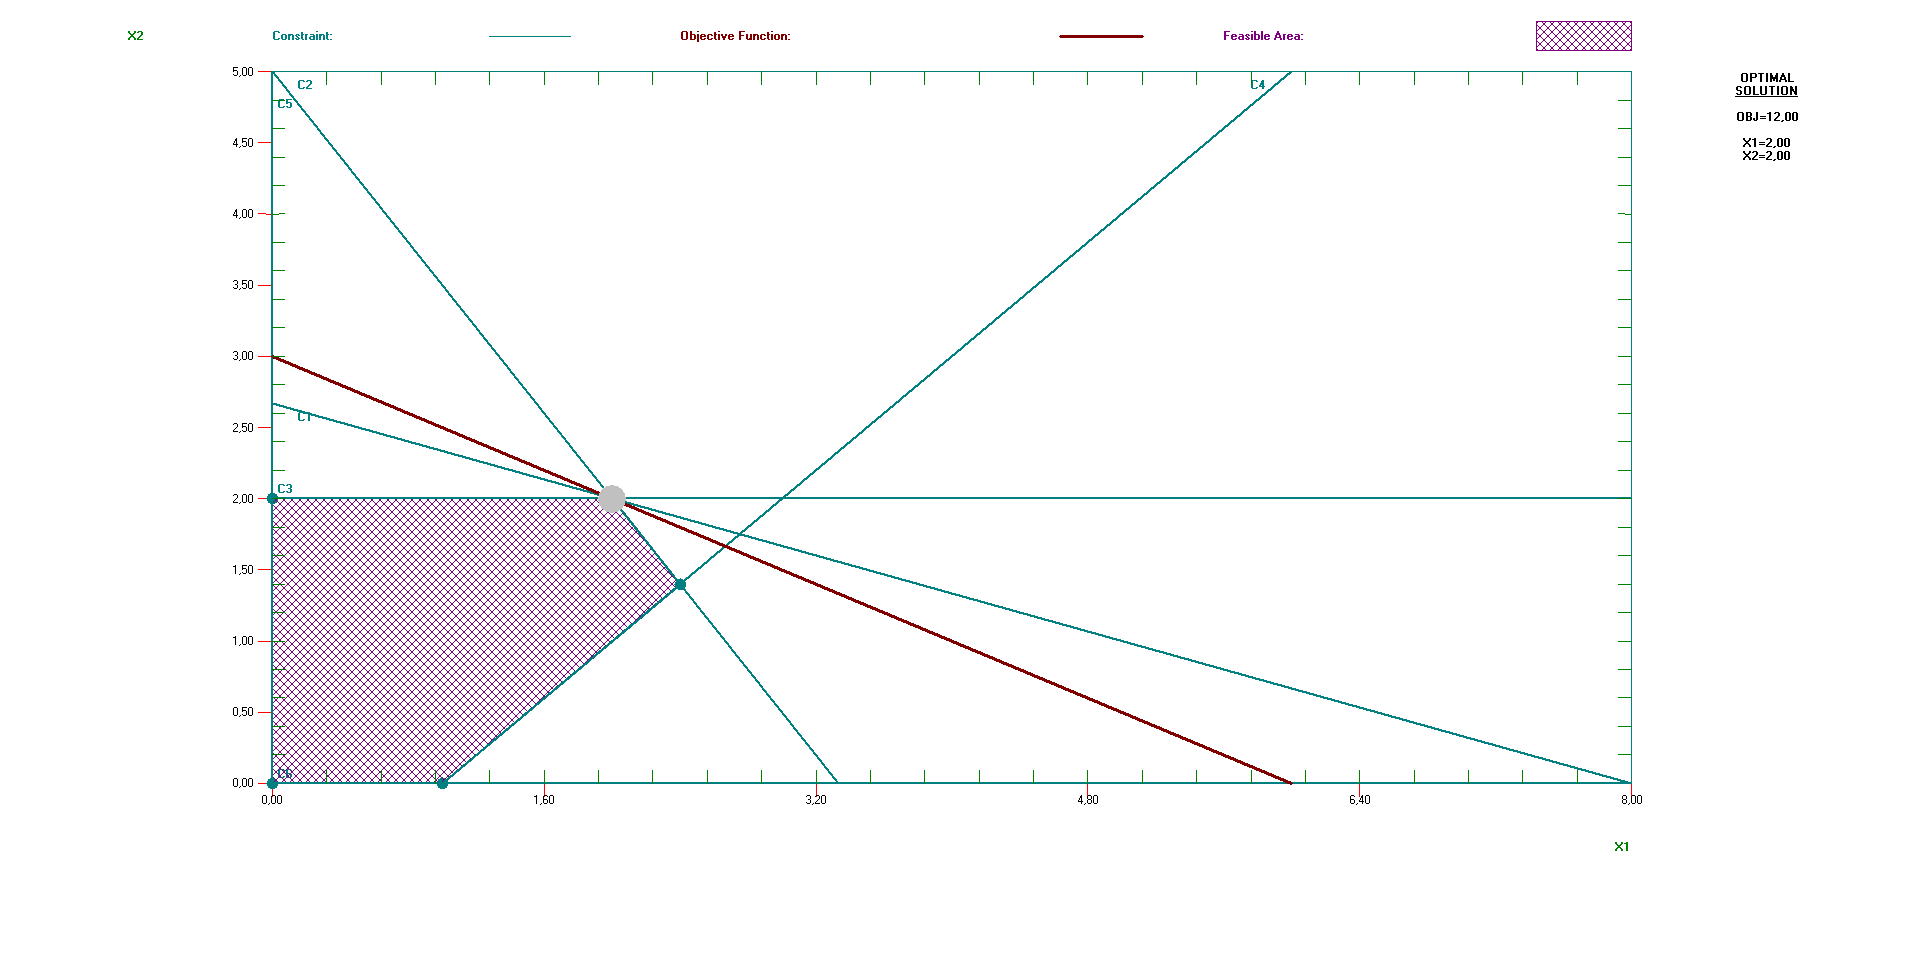
\includegraphics[width=18cm]
  {inc/result1_option1.png}

  \caption{Задание 1 вариант 1}
  \label{fig:result1_option1}
\end{figure}


\textbf{Ответ}: $x_1 = 2$; $x_2 = 2$, $y_{max} = 12$.

\newpage

\begin{center}
  \textbf{Задание 2}
\end{center}

\textbf{Условие}:

Для доставки горюче-смазочных материалов в порт нефтеперерабатывающий завод располагает тремя типами транспортных средств.
Количество транспортных средств различных типов и их производительность по числу заправок,
перевозимых в единицу времени, показаны на рисунке~\ref{fig:task2_1}.

\begin{figure}[!htb]
  \centering

  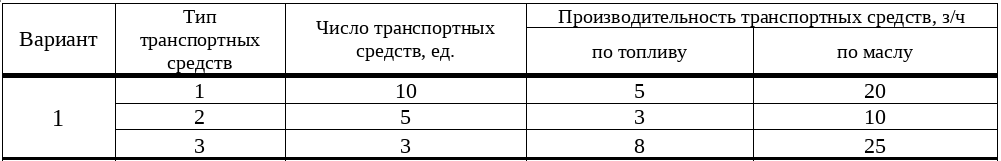
\includegraphics[width=16cm]
  {inc/task2_1.png}

  \caption{Задание 2 вариант 1}
  \label{fig:task2_1}
\end{figure}

Найти план использования транспортных средств,
обеспечивающий доставку горюче смазочных материалов по числу заправок
с учетом комплектности их доставки?

\textbf{Решение}:

$x_1$ - количество транспортных средств типа 1;

$x_2$ - количество транспортных средств типа 2;

$x_3$ - количество транспортных средств типа 3.

$$
\begin{cases}
  x_1  \leq 10 & \text{- количество транспортных средств типа 1}\\
  x_2 \leq 5   & \text{- количество транспортных средств типа 2}\\
  x_3 \leq 3   & \text{- количество транспортных средств типа 3}\\
  5 x_1 + 2 x_2 + 8 x_3 &\text{- производительность транспортных средств по топливу}\\
  20 x_1 + 10 x_2 + 25 x_3 &\text{- производительность транспортных средств по маслу}\\
  x_1 \geq 0, x_2 \geq 0, x_3 \geq 0 &\text{- условие не отрицательности переменной}
\end{cases}
$$

\textbf{Ответ}: $\emptyset$ (нет решений, так как нельзя составить целевую функцию).

\newpage

\begin{center}
  \textbf{Задание 3}
\end{center}

\textbf{Условие}:

Фирма «ПОЛЮСТРОВО» производит два безалкогольных широко популярных напитка «Колокольчик» и «Буратино».
Для производства одного литра «Колокольчика» требуется времени работы оборудования t1,
а для «Буратино» - t2.
Расход специальных ингредиентов на них составляет $t_1$ и $t_2$ на один литр соответственно.
Ежедневно в распоряжении фирмы $\beta$ специального ингредиента и $\delta$ смен работы оборудования.
Доход от продажи одного литра напитка составляет $d_1$ и $d_2$ соответственно.

Определите ежедневный план производства напитков каждого вида,
обеспечивающий максимальный доход от их продажи?

Исходные данные представлены на рисунке~\ref{fig:task3_1}.

\begin{figure}[!htb]
  \centering

  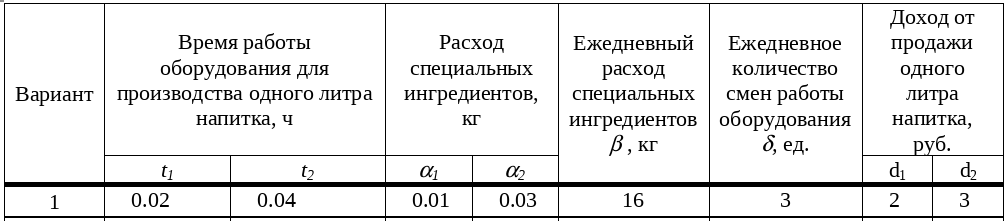
\includegraphics[width=16cm]
  {inc/task3_1.png}

  \caption{Задание 3 вариант 1}
  \label{fig:task3_1}
\end{figure}


\textbf{Решение}:

$x_1$ - количество литров напитка <<Колокольчик>>;

$x_2$ - количество литров напитка <<Буратино>>.

$$
\begin{cases}
  y = 2 x_1 + 3 x_2 \implies max &\text{- ежедневный доход от продажи}\\
  0.01 x_1 + 0.03 x_2 \leq 16 &\text{- ограничение для ежедневного расходы сырья A}\\
  0.02 x_1 + 0.04 x_2 \leq 8.3 &\text{- ограничение для ежедневного расходы сырья B}\\
  x_1 \geq 0, x_2 \geq 0 &\text{- условие не отрицательности переменной}
\end{cases}
$$

\begin{center}
  \textbf{Решение системы через WinQSB}
\end{center}

На VirtualBox \cite{VirtualBox} устанавливаем WinXP \cite{WinXP}, а на неё программу WinSQB \cite{WinQSB}.

Пуск > WinQSB > Linear and Integer Programming > File > New Problem

Problem Title: MO.PO4.190333-01\_03

Number of Variables: 2

Number of Constraints: 4

Object Criterion > Maxamization

OK> Заполняем таблицу (см.таблицу~\ref{tab:3_5})

\begin{table}[h!]
  %\scriptsize

  \centering

  \caption{Решение задачи №3.5 в WinQSB (Linear and Integer Programming)}
  \label{tab:3_5}

  \begin{tabular}{ |l||c|c|c|c| } 
    \hline
    Variable & X1 & X2 & Direction & R. H. S \\ \hline
    \hline
    Maximaze & 2 & 3 &  & \\ \hline
    C1 & 0.01 & 0.03 & <= & 16 \\ \hline
    C2 & 0.02 & 0.04 & <= & 24 \\ \hline
    C3 & 1 & 0 & >= & 0 \\ \hline
    C4 & 0 & 1 & >= & 0 \\ \hline
    %LowerBound & 0 & 0 &  & \\ \hline
    %UpperBound & M & M &  & \\ \hline
    %VariableType & Continious & Continious &  & \\ \hline
  \end{tabular}
\end{table}

Жмем розовую кнопку > ОК

Options > Change XY Ranges and Colors > Background (жмем, пока не получим белый цвет) > ОК

Options > Change XY Variables > OK

File > Save As > 3.bmp. Результат на рисунке~\ref{fig:result3_option1}.

\begin{figure}[!htb]
  \centering

  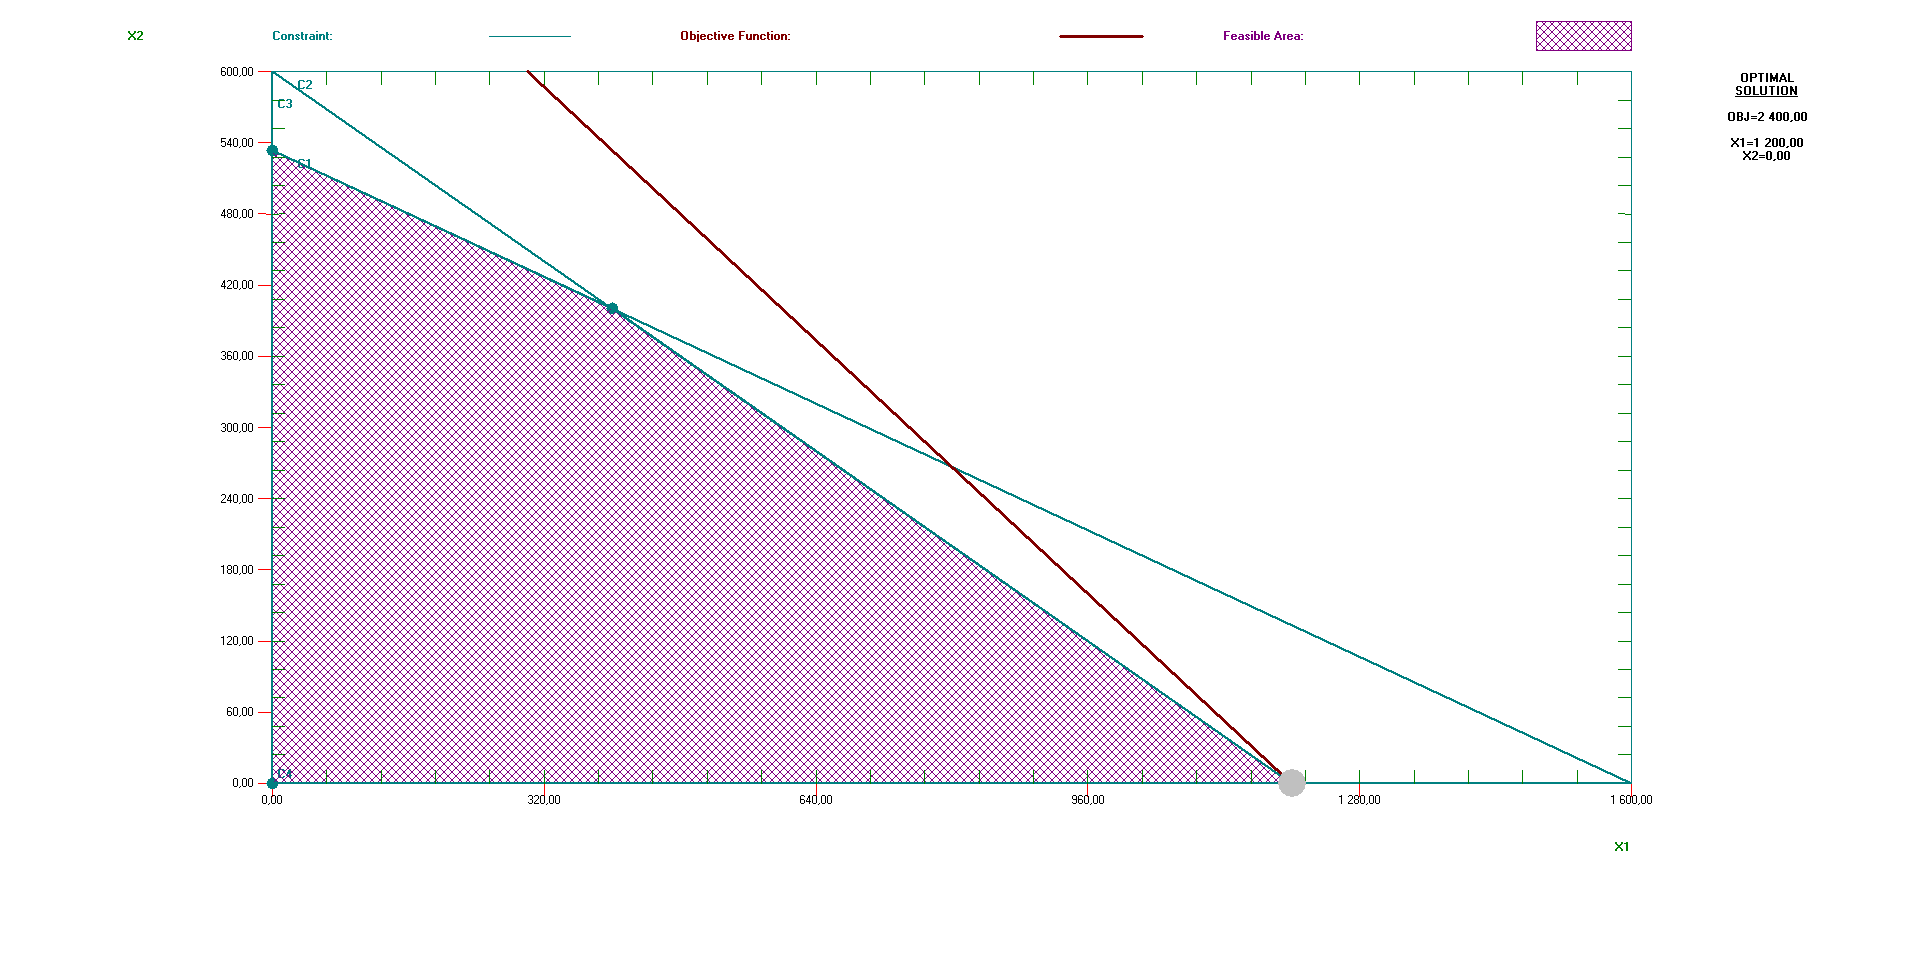
\includegraphics[width=18cm]
  {inc/result3_option1.png}

  \caption{Задание 3 вариант 1}
  \label{fig:result3_option1}
\end{figure}

\textbf{Ответ}: $x_1 = 1200$; $x_2 = 0$, $y_{max} = 2400$.

\newpage

\begin{center}
  \textbf{Задание 4}
\end{center}

\textbf{Условие}:

Туристическая фирма, располагая флотилией из двух типов судов,
в летний сезон обслуживает в среднем $\eta$ туристов.
В месяц выделяется $\varphi$ т. топлива.
Потребность в рабочей силе не превышает k человек.

Определить эффективное количество судов первого и второго типа для обеспечения максимального дохода,
который составляет от эксплуатации судов первого типа $\alpha_1$ млн. руб.,
а судов второго типа – $\alpha_2$ млн. руб.?

Исходные данные представлены на рисунке~\ref{fig:task4_1}.

\begin{figure}[!htb]
  \centering

  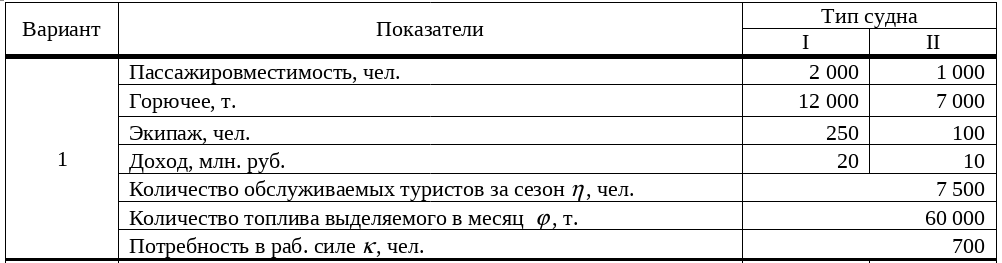
\includegraphics[width=16cm]
  {inc/task4_1.png}

  \caption{Задание 4 вариант 1}
  \label{fig:task4_1}
\end{figure}

\textbf{Решение}:

$x_1$ - количество судов типа I;

$x_2$ - количество судов типа II.

$$
\begin{cases}
  y = 20 x_1 + 10 x_2 \implies max &\text{- общий доход}\\
  2000 x_1 + 1000 x_2 \leq 80 &\text{- ограничение количества обслуживаемых туристов}\\
  12000 x_1 + 7000 x_2 \leq 70 &\text{- ограничение на количество топлива}\\
  250 x_1 + 100 x_2 \leq 30 &\text{- потребность в рабочей силе}\\
  x_1 \geq 0, x_2 \geq 0 &\text{- условие не отрицательности переменной}\\
  &\text{  (количество судна не может быть отрицательным)}
\end{cases}
$$

\begin{center}
  \textbf{Решение системы через WinQSB}
\end{center}

На VirtualBox \cite{VirtualBox} устанавливаем WinXP \cite{WinXP}, а на неё программу WinSQB \cite{WinQSB}.

Пуск > WinQSB > Linear and Integer Programming > File > New Problem

Problem Title: MO.PO4.190333-01\_04

Number of Variables: 2

Number of Constraints: 5

Object Criterion > Maxamization

OK> Заполняем таблицу (см.таблицу~\ref{tab:4_5})

\begin{table}[h!]
  %\scriptsize

  \centering

  \caption{Решение задачи №4.5 в WinQSB (Linear and Integer Programming)}
  \label{tab:4_5}

  \begin{tabular}{ |l||c|c|c|c| } 
    \hline
    Variable & X1 & X2 & Direction & R. H. S \\ \hline
    \hline
    Maximaze & 20 & 10 &  & \\ \hline
    C1 & 2000 & 1000 & <= & 7500 \\ \hline
    C2 & 12000 & 1000 & <= & 60000 \\ \hline
    C3 & 250 & 100 & <= & 700 \\ \hline
    C4 & 1 & 0 & >= & 0 \\ \hline
    C5 & 0 & 1 & >= & 0 \\ \hline
    %LowerBound & 0 & 0 &  & \\ \hline
    %UpperBound & M & M &  & \\ \hline
    %VariableType & Continious & Continious &  & \\ \hline
  \end{tabular}
\end{table}

Жмем розовую кнопку > ОК

Options > Change XY Ranges and Colors > Background (жмем, пока не получим белый цвет) > ОК

Options > Change XY Variables > OK

File > Save As > 4.bmp. Результат на рисунке~\ref{fig:result4_option1}.

\begin{figure}[!htb]
  \centering

  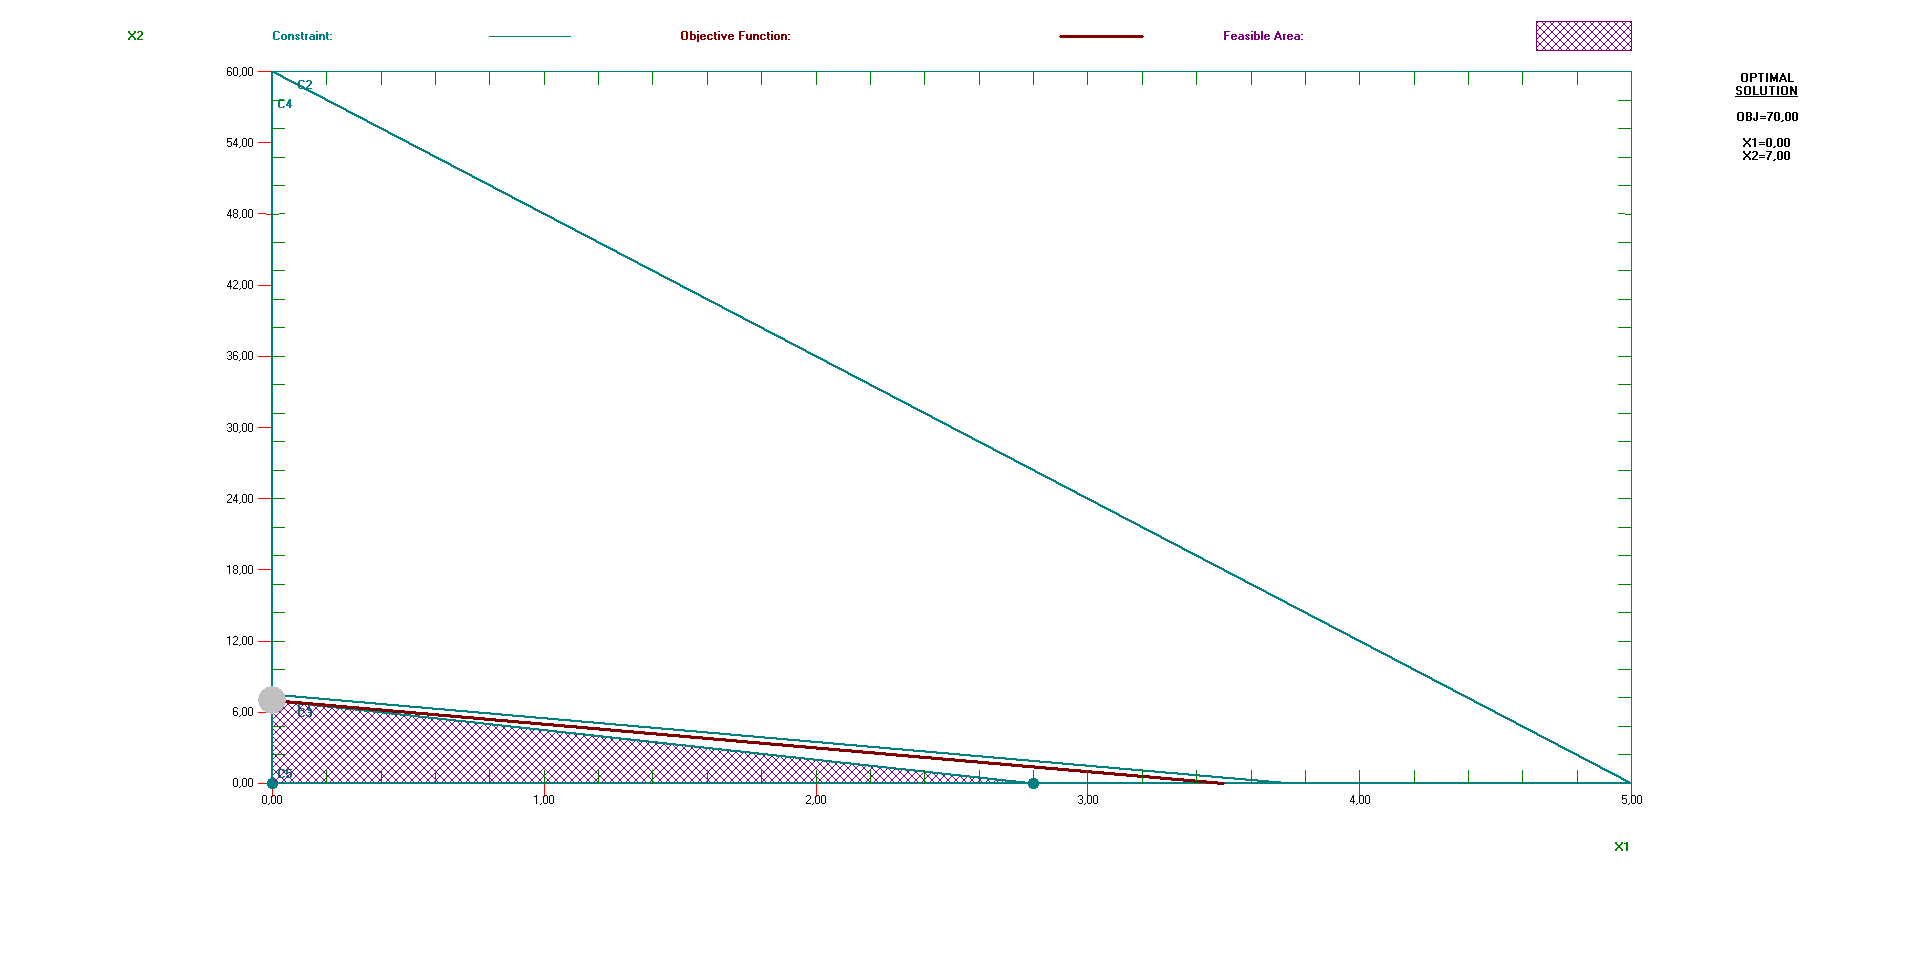
\includegraphics[width=18cm]
  {inc/result4_option1.png}

  \caption{Задание 4 вариант 1}
  \label{fig:result4_option1}
\end{figure}

\textbf{Ответ}: $x_1 = 0$; $x_2 = 7$, $y_{max} = 70$.

\newpage

\begin{center}
  \textbf{Задание 5}
\end{center}

\textbf{Условие}:

С Московского вокзала Санкт-Петербурга ежедневно на Москву отправляются скорые и пассажирские поезда.
Количество различных типов вагонов железнодорожного депо станции отправления
и их пассажировместимость указаны на рисунке~\ref{fig:task5_1}.

\begin{figure}[!htb]
  \centering

  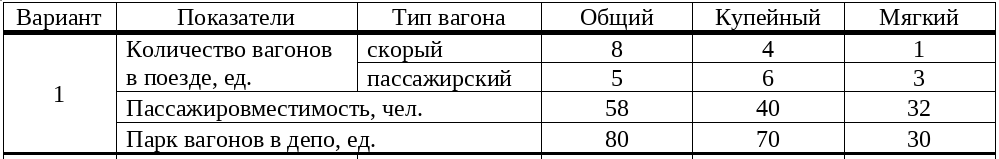
\includegraphics[width=16cm]
  {inc/task5_1.png}

  \caption{Задание 5 вариант 1}
  \label{fig:task5_1}
\end{figure}

Определить количество пассажирских и скорых поездов,
обеспечивающих перевозку максимального количества пассажиров.


\textbf{Решение}:

$x_1$ - количество скоростных поездов;

$x_2$ - количество пассажирских поездов.

$n_1 = 58\cdot 8 + 40\cdot 4 + 32\cdot 1 = 304 + 160 + 32 = 496$ - пассажировместимость скорого поезда;

$n_2 = 58\cdot 5 + 40\cdot 6 + 32\cdot 3 = 290 + 240 + 96 = 626$ - пассажировместимость пассажирского.

$$
\begin{cases}
  y = 496 x_1 + 626 x_2 \implies max &\text{- ежедневный доход от продажи}\\
  8 x_1 + 5 x_2 \leq 80 &\text{- ограничение на общее количество вагонов в депо}\\
  4 x_1 + 6 x_2 \leq 70 &\text{- ограничение на купейное количество вагонов в депо}\\
  1 x_1 + 3 x_2 \leq 30 &\text{- ограничение на мягкие количество вагонов в депо}\\
  x_1 \geq 0, x_2 \geq 0 &\text{- условие не отрицательности переменной}
\end{cases}
$$

\begin{center}
  \textbf{Решение системы через WinQSB}
\end{center}

На VirtualBox \cite{VirtualBox} устанавливаем WinXP \cite{WinXP}, а на неё программу WinSQB \cite{WinQSB}.

Пуск > WinQSB > Linear and Integer Programming > File > New Problem

Problem Title: MO.PO4.190333-01\_05

Number of Variables: 2

Number of Constraints: 5

Object Criterion > Maxamization

OK> Заполняем таблицу (см.таблицу~\ref{tab:5_5})

\begin{table}[p!]
  %\scriptsize

  \centering

  \caption{Решение задачи №5.5 в WinQSB (Linear and Integer Programming)}
  \label{tab:5_5}

  \begin{tabular}{ |l||c|c|c|c| } 
    \hline
    Variable & X1 & X2 & Direction & R. H. S \\ \hline
    \hline
    Maximaze & 496 & 626 &  & \\ \hline
    C1 & 8 & 5 & <= & 80 \\ \hline
    C2 & 4 & 6 & <= & 70 \\ \hline
    C3 & 1 & 30 & <= & 30 \\ \hline
    C4 & 1 & 0 & >= & 0 \\ \hline
    C5 & 0 & 1 & >= & 0 \\ \hline
    %LowerBound & 0 & 0 &  & \\ \hline
    %UpperBound & M & M &  & \\ \hline
    %VariableType & Continious & Continious &  & \\ \hline
  \end{tabular}
\end{table}

Жмем розовую кнопку > ОК

Options > Change XY Ranges and Colors > Background (жмем, пока не получим белый цвет) > ОК

Options > Change XY Variables > OK

File > Save As > 5.bmp. Результат на рисунке~\ref{fig:result5_option1}.

\begin{figure}[p!]
  \centering

  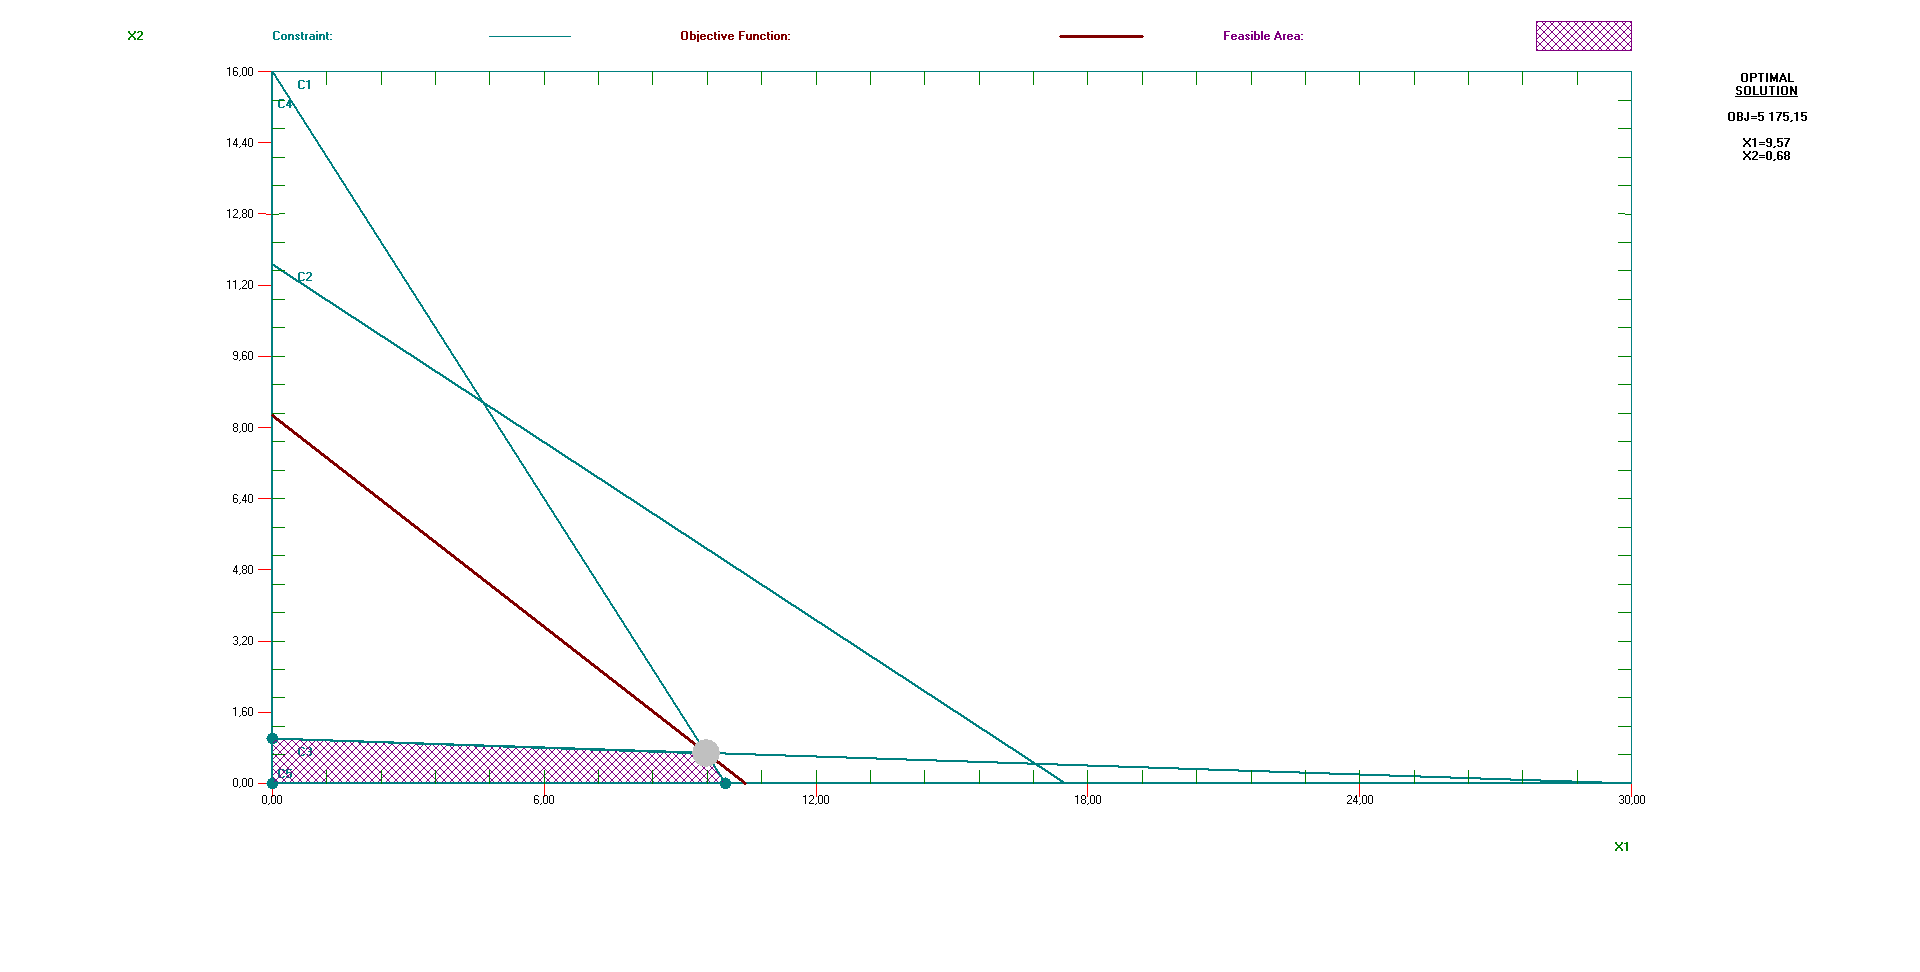
\includegraphics[width=18cm]
  {inc/result5_option1.png}

  \caption{Задание 5 вариант 1}
  \label{fig:result5_option1}
\end{figure}

\textbf{Ответ}: $x_1 = 4.74$; $x_2 = 8.82$, $y_{max} = 7621.05$.

% \begin{center}
%   \textbf{Вариант 5}
% \end{center}
% 
% $$
% \mathbb{Z} = -2 x +2 y
% $$
% 
% $$
% \begin{cases}
%   4x - 3 y  \leq 12\\
%   x + y \leq 10 \\
%   2 x + y \geq 6\\
%   x \geq 0, y \geq 0
% \end{cases}
% $$
% 
% \textbf{Решение}:
% 
% \subparagraph{1}
% Построим область допустимых значений.
% Сразу начертим систему координат.
% В задаче будут приниматься переменные x и y.
% 
% \subparagraph{1.1}
% Начнём с первой линии.
% Если неравенство ($4x - 3 y  \leq 12$) заменить знаком равно, то это будет уравнение прямой ($4x - 3 y  = 12$).
% Прямую можно построить по двум точкам.
% Для простоты x примем за 0, потом y.
% 
% $
% \text{if } x = 0 \implies 4 \cdot 0 - 3 y = 12, -3y = 12, y=-4
% $
% 
% $
% \text{if } y = 0 \implies 4 x - 3 \cdot 0 = 12, 4x=12, x=3
% $
% 
% Отметим точку (0; -4) и (0; 2) на графике.
% Соединим точки прямой линией.
% Теперь вспомним, что выражению ($4x - 3 y  \leq 12$) соответствует знак меньше или равно
% - и определим какой из областей под ней или над ней нужно заштриховать.
% Для простоты возьмем начало координат: точку O(0; 0)
% и посмотрим удовлетворяет ли она неравенству ($4x - 3 y  \leq 12$).
% 
% $
% 4 \cdot 0 - 3 \cdot 0  \leq 12, 0 \leq 12 \implies \text{верно} \implies \text{O(0; 0)} \in (4x-3y\leq 12)
% $
% 
% Значит точка O(0; 0) принадлежит области, значит заштрихована будет та область, в которой лежит точка O(0; 0).
% 
% Результат смотри на рисунке~\ref{fig:1}.
% 
% % = = = = =
% 
% \subparagraph{1.2}
% Теперь тоже самое проделаем и со вторым условием ($x+y \leq 10$)
% Если неравенство ($x+y \leq 10$) заменить знаком равно, то это будет уравнение прямой ($x+y = 10$).
% Прямую можно построить по двум точкам.
% Для простоты x примем за 0, потом y.
% 
% $
% \text{if } x = 0 \implies 0+y=10, y=10
% $
% 
% $
% \text{if } y = 0 \implies x+0=10, x=10
% $
% 
% Отметим точку (0; 19) и (10; 0) на графике.
% Соединим точки прямой линией.
% Теперь вспомним, что выражению ($x+y \leq 10$) соответствует знак меньше или равно
% - и определим какой из областей под ней или над ней нужно заштриховать.
% Для простоты возьмем начало координат: точку O(0; 0)
% и посмотрим удовлетворяет ли она неравенству ($x+y \leq 10$).
% 
% $
% 0+0 \leq 10, 0 \leq 10 \implies \text{верно} \implies \text{O(0; 0)} \in (x+y\leq 10)
% $
% 
% Значит точка O(0; 0) принадлежит области, значит заштрихована будет та область, в которой лежит точка O(0; 0).
% 
% Результат смотри на рисунке~\ref{fig:2}.
% 
% \subparagraph{1.3}
% Теперь тоже самое проделаем и с третьим условием ($2x+y \geq 6$)
% Если неравенство ($2x+y \geq 6$) заменить знаком равно, то это будет уравнение прямой ($2x+y = 6$).
% Прямую можно построить по двум точкам.
% Для простоты x примем за 0, потом y.
% 
% $
% \text{if } x = 0 \implies 2\cdot0+y=6, y=6
% $
% 
% $
% \text{if } y = 0 \implies 2x+0=6, 2x=6, x=3
% $
% 
% Отметим точку (0; 6) и (3; 0) на графике.
% Соединим точки прямой линией.
% Теперь вспомним, что выражению ($2x+y \geq 6$) соответствует знак больше или равно
% - и определим какой из областей под ней или над ней нужно заштриховать.
% Для простоты возьмем начало координат: точку O(0; 0)
% и посмотрим удовлетворяет ли она неравенству ($2x+y \geq 6$).
% 
% $
% 2\cdot0+0 \geq 6, 0 \geq 6 \implies \text{ложь} \implies \text{O(0; 0)} \notin (2x+y \geq 6)
% $
% 
% Значит точка O(0; 0) не принадлежит области, значит заштрихована будет та область, в которой нет точки O(0; 0).
% 
% Результат смотри на рисунке~\ref{fig:3}.
% 
% \begin{figure}[!htb]\centering
%   \begin{minipage}{0.32\textwidth}
%     \centering
% 
%     \includegraphics[width=0.99\textwidth]
%     {inc/1.eps}
%   
%     \caption{Область $(4x-3y\leq 12)$}
% 
%     \label{fig:1}
%   \end{minipage}
%   \begin{minipage}{0.32\textwidth}
%     \centering
% 
%     \includegraphics[width=0.99\textwidth]
%     {inc/2.eps}
%   
%     \caption{Область $(x+y\leq 10)$}
% 
%     \label{fig:2}
%   \end{minipage}
%   \begin{minipage}{0.32\textwidth}
%     \centering
% 
%     \includegraphics[width=0.99\textwidth]
%     {inc/3.eps}
%   
%     \caption{Область $(2x+y\geq 6)$}
% 
%     \label{fig:3}
%   \end{minipage}
% \end{figure}
% 
% \subparagraph{2}
% Для удобства нарисуем новый график.
% Раскрасим его цветами.
% Учитывая, что существует условие не отрицательности переменной,
% заштрихуем получившуюся область.
% 
% Теперь в этой области нужно найти точку,
% в которой функция $\mathbb{Z}$ принимает максимальное и минимальное значение.
% 
% $\mathbb{Z} =-2x+2x \to \text{max, min}$
% 
% Если мы запишем градиент функции, то это будет вектор, координатами которого будет частные производные функции.
% 
% $\text{grad }\mathbb{Z} = \{-2; 2\} = \bar{c}$
% 
% Он называется условным вектором и показывает направление максимального роста функции.
% 
% Общий график смотри на рисунке~\ref{fig:456}.
% 
% \begin{figure}[!htb]\centering
%   \begin{minipage}{0.32\textwidth}
%     \centering
% 
%     \includegraphics[width=0.99\textwidth]
%     {inc/4.eps}
%   \end{minipage}
%   \begin{minipage}{0.32\textwidth}
%     \centering
% 
%     \includegraphics[width=0.99\textwidth]
%     {inc/5.eps}
%   \end{minipage}
%   \begin{minipage}{0.32\textwidth}
%     \centering
% 
%     \includegraphics[width=0.99\textwidth]
%     {inc/6.eps}
%   \end{minipage}
%   \caption{Общий график}
%   \label{fig:456}
% \end{figure}
% 
% Начертим этот вектор на графике. Теперь проведем вектору $\bar{c}$ перпендикуляр
% и будем параллельно двигать в сторону вектора $\bar{c}$,
% направления роста функции,
% пока он не достигнет крайнего значения области.
% 
% И так мы дошли до крайнего значения области (-3; 0) - для max и (0; 10) - для min.
% 
% Значит в точке (3;0) - функция достигает максимума,
% в точке (0;10) - функция достигает минимума.
% 
% $\mathbb{Z}_{max}$ - это значение в точке (3; 0).
% 
% $\mathbb{Z}_{min}$ - это значение в точке (0; 10).
% 
% $\mathbb{Z}_{max} = \mathbb{Z}(3; 0) = -2\cdot 3 + 2\cdot 0 = -6$
% 
% $\mathbb{Z}_{min} = \mathbb{Z}(0; 10) = -2\cdot 0 + 2 \cdot 10 = 20$
% 
% \subparagraph{} \textbf{Ответ}: $\mathbb{Z}_{max} = \mathbb{Z}(3;0)=-6$, $\mathbb{Z}_{min} = \mathbb{Z}(0; 10) = 20$.
% 
% \newpage
% 
% \begin{center}
% \textbf{Проверка max через WinQSB}
% \end{center}
% 
% На VirtualBox \cite{VirtualBox} устанавливаем WinXP \cite{WinXP}, а на неё программу WinSQB \cite{WinSQB}.
% 
% Пуск > WinQSB > Linear and Integer Programming > File > New Problem
% 
% Problem Title: MO\_PO4\_190333\_00\_max
% 
% Number of Variables: 2
% 
% Number of Constraints: 3
% 
% Object Criterion > Maxamization
% 
% OK> Заполняем таблицу
% 
% \begin{table}[h!]
%   \centering
%   \begin{tabular}{ |l||c|c|c|c| } 
%     \hline
%     Variable & X1 & X2 & Direction & R. H. S \\ \hline
%     \hline
%     Maximaze & -2 & 2 &  & \\ \hline
%     C1 & 4 & -3 & <= & 12 \\ \hline
%     C2 & 1 & 1 & <= & 10 \\ \hline
%     C3 & 2 & 1 & >= & 6 \\ \hline
%     LowerBound & 0 & 0 &  & \\ \hline
%     UpperBound & M & M &  & \\ \hline
%     VariableType & Continious & Continious &  & \\ \hline
%   \end{tabular}
% \end{table}
% 
% Жмем розовую кнопку > ОК
% 
% Options > Change XY Ranges and Colors > Background (жмем, пока не получим белый цвет) > ОК
% 
% Options > Change XY Variables > OK
% 
% File > Save As > 1.bmp. Результат на рисунке~\ref{fig:max}.
% 
% \begin{figure}[!htb]
%   \centering
% 
%   \includegraphics[width=16cm]
%   {inc/max.png}
% 
%   \caption{Ищем max через WinSQB}
%   \label{fig:max}
% \end{figure}
% 
% \textbf{Вывод}: Получили в программе 20. Ручным способом получили 20. Результаты равны, значит решили верно.
% 
% \newpage
% 
% \begin{center}
% \textbf{Проверка min через WinQSB}
% \end{center}
% 
% На VirtualBox \cite{VirtualBox} устанавливаем WinXP \cite{WinXP}, а на неё программу WinSQB \cite{WinSQB}.
% 
% Пуск > WinQSB > Linear and Integer Programming > File > New Problem
% 
% Problem Title: MO.PO4.190333-00\_min
% 
% Number of Variables: 2
% 
% Number of Constraints: 3
% 
% Object Criterion > Minimization
% 
% OK> Заполняем таблицу
% 
% \begin{table}[h!]
%   \centering
%   \begin{tabular}{ |l||c|c|c|c| } 
%     \hline
%     Variable & X1 & X2 & Direction & R. H. S \\ \hline
%     \hline
%     Minimize & -2 & 2 &  & \\ \hline
%     C1 & 4 & -3 & <= & 12 \\ \hline
%     C2 & 1 & 1 & <= & 10 \\ \hline
%     C3 & 2 & 1 & >= & 6 \\ \hline
%     LowerBound & 0 & 0 &  & \\ \hline
%     UpperBound & M & M &  & \\ \hline
%     VariableType & Continious & Continious &  & \\ \hline
%   \end{tabular}
% \end{table}
% 
% Жмем розовую кнопку > ОК
% 
% Options > Change XY Ranges and Colors > Background (жмем, пока не получим белый цвет) > ОК
% 
% Options > Change XY Variables > OK
% 
% File > Save As > 1.bmp. Результат на рисунке~\ref{fig:min}.
% 
% \begin{figure}[!htb]
%   \centering
% 
%   \includegraphics[width=16cm]
%   {inc/min.png}
% 
%   \caption{Ищем min через WinSQB}
%   \label{fig:min}
% \end{figure}
% 
% \textbf{Вывод}: Получили в программе -6. Ручным способом получили -6. Результаты равны, значит решили верно.
% 